% colors from http://colorbrewer2.org/?type=sequential&scheme=Blues&n=3
\definecolor{blue1}{HTML}{DEEBF7}
\definecolor{blue2}{HTML}{9ECAE1}
\definecolor{blue3}{HTML}{3182BD}
\definecolor{green1}{HTML}{E5F5E0}
\definecolor{green2}{HTML}{A1D99B}
\definecolor{green3}{HTML}{31A354}

\begin{figure}[t]
\centering
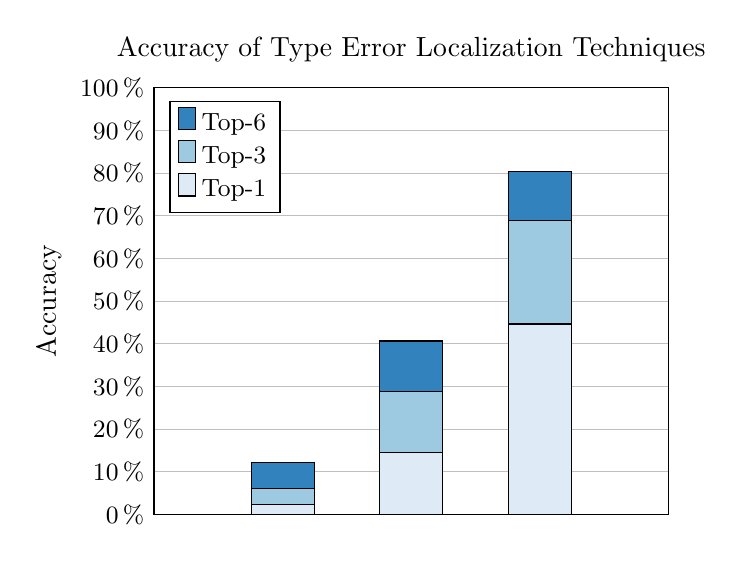
\begin{tikzpicture}
\begin{axis}[
  ybar stacked,
  % width=\linewidth,
  height=7cm,
  title={Accuracy of Type Error Localization Techniques},
  ylabel={Accuracy},
  bar width=0.8cm,
  ymin=0.0,
  ymax=100.0,
  ytick={0.0, 10.0, 20.0, 30.0, 40.0, 50.0, 60.0, 70.0, 80.0, 90.0, 100.0},
  yticklabel={\pgfmathparse{\tick}\pgfmathprintnumber{\pgfmathresult}\,\%},
  ytick style={draw=none},
  ymajorgrids = true,
  symbolic x coords={random, popular, dnn},
  enlarge x limits=0.5,
  xtick=data,
  xtick style={draw=none},
  xticklabels={\random, \popular, \dnn},
  %x tick label style={rotate=45, anchor=north east},
  x tick label style={font=\small},
  y tick label style={font=\small},
  reverse legend,
  transpose legend,
  legend style={legend pos = north west, legend columns=4, font=\small},
]

\addplot[draw=black, fill=blue1] coordinates {(random, 2.35646958011996552) (popular, 14.438731790916881) (dnn, 44.64438731790917)};
\addlegendentry{Top-1}
\addplot[draw=black, fill=blue2] coordinates {(random, 3.6846615252784924) (popular, 14.395886889460153) (dnn, 24.250214224507282)};
\addlegendentry{Top-3}
\addplot[draw=black, fill=blue3] coordinates {(random, 6.212510711225363) (popular, 11.825192802056556) (dnn, 11.482433590402735)};
\addlegendentry{Top-6}

%%% TODO: Maybe add a random forest? or a smaller DNN? those dont achieve the same accuracy...

\end{axis}
\end{tikzpicture}
\caption{
  Results of our template prediction classifiers using the \emph{50 most
  popular} templates. We present the results up to the top 6 predictions, since
  our synthesis algorithm considers that many templates before falling to a
  different location. Our classifiers were trained on the \SPRING quarter and
  evaluated on the \FALL quarter of an undergraduate Programming Languages
  course.
}
\label{fig:accuracy-results}
\end{figure}
